\chapter{Evaluations and Performances}\label{chap:perfs}

\section{Test application}\label{sec:vpnapp}

MPDTLS is implemented inside a library, we thus need a suitable application to use this library. We tried to find out which application could be a good candidate for our tests. First, we needed an application which uses DTLS for most of its communications and is open source. It was surprisingly hard to find but we still managed to find one : Campagnol\cite{campagnol}. Campagnol is a decentralized VPN solution which is using DTLS to communicate between the peers. Unfortunately, for a set of reasons exposed in Appendix \ref{app:campagnol}, we were unable to integrate correctly our modified library within the application. 

So, we took the decision to build our own VPN application \cite{wolfssl-vpn} and reuse part of Campagnol's code. A VPN application is indeed perfectly suitable for all the experiences we could imagine : potentially any application can use a VPN tunnel without even noticing it. Every packet is encapsulated inside a DTLS packet transmitted securely between the two MPDTLS hosts (see Figure \ref{fig:vpn}).

\begin{figure}[!ht]
\centering
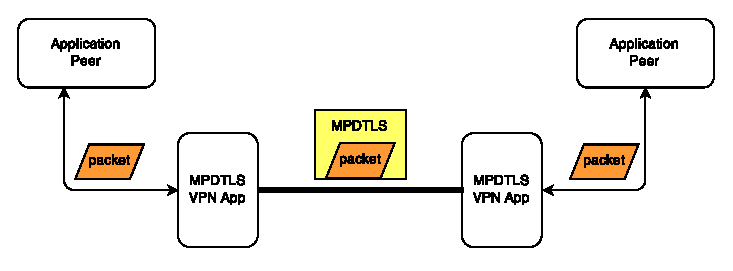
\includegraphics{images/vpn.eps}
\caption{A simple VPN application using MPDTLS}
\label{fig:vpn}
\end{figure}

The behavior of one of this MPDTLS VPN App is shown on Figure \ref{fig:vpn-io}. A TUN interface is created with a specified address and netmask. Every packet going to an address falling in this netmask will be sent by the kernel to this interface. What we need then is to monitor this interface, read the packets that have arrived and sent them through the tunnel. This is the job of the first thread (in red on the Figure). We also need to capture packets coming from the network and write them in the TUN interface. This is handled by a second thread represented in green on the Figure. Finally, a last thread (in blue) is listening the standard input for potential commands. This is the channel we use to communicate with the application to add or remove new interfaces for instance. We can ask for debug information or even change the scheduler policy on the fly.

\begin{figure}[!ht]
\centering
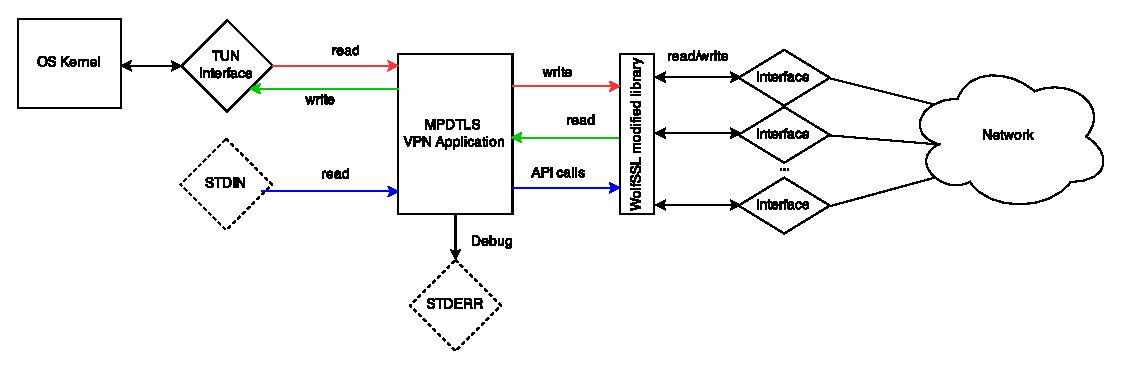
\includegraphics[width=\textwidth]{images/tunneling-IO.eps}
\caption[I/O interactions for one host of our application]{I/O interactions for one host of our application. Each thread is represented with one color.} 
\label{fig:vpn-io}
\end{figure}

One of the most useful information we can ask for are the statistics for a particular flow. Just by looking at this output, we can most of the time identify a problem without even looking at the Wireshark trace. An example of such an output is shown on Listing \ref{lst:stats}. We can easily see the part of traffic the flow is actually supporting, the estimated delays and other information. The separator | is used in the packets sent list to differentiate the ones that are in the waiting state and the others (see Section \ref{sec:impl-stats} for more details about this waiting state).

\begin{lstlisting}[language=bash,caption=An output of the statistics for a particular flow,label=lst:stats]
---- Stats Flow N 0 ---- 
IP src : 11.0.0.1 
IP dst : 11.2.0.1 
Support 41 % of the connection
----- Receiver Stats ----- 
Packets received : 44 
Min_Seq received : 76 
Max_Seq received : 172 
Backward delay : 10 ms
----- Receiver Cache ----- 
Packets received : 0 
Min_Seq received : 2147483647 
Max_Seq received : 0 
----- Sender Stats ----- 
Packets sent : [ 8487 8489 8492 ... 8633 8634 8636 | 8640 8642 ... 8706 8707] 
Forward delay : 10 ms
Loss Rate : 0.000000 
---------------------------

\end{lstlisting}

\section{Different scheduler policies}\label{sec:perf-sched}

We present here the different scheduler strategies we have implemented and how the fractional distribution is computed in each case. At the end each of them has pros and cons, the good choice is strongly related with what the underlying application expect to do. It may even be needed that an application has to build its own scheduler and that is perfectly fine with our design since we have a dedicated callback.

\subsection{Round Robin}

The round robin is the simplest strategy consisting in giving the same amount of traffic to each of the available links. This does not use any of the information gathered with the feedback. However it may be a good choice if we know in advance that the different links are sharing common properties (e.g. in a datacenter).

The fractional distribution is really easy to compute as every link will get the same fraction of traffic.

\begin{equation*}
f_i = \frac{1}{n}
\end{equation*}

where $f_i$ is the portion of traffic given to flow $i$ and $n$ is the total number of flows.

\subsection{Optimize Latency}

For this strategy, we want to give more weight to links where the forward delay is lower. We have to keep in mind that in every delay $d_i$, we have the clock desynchronization term (see Section \ref{sec:forward-delay}). In order to get rid of this term, we must consider the difference with another delay. We choose to take the difference with the maximum delay as by definition the greater the difference, the smaller the delay. Equation \ref{eq:latency} gives the complete expression.  

\begin{equation}
f_i = \frac{max_d - d_i + \alpha}{\sum_j (max_d - d_j) + n*\alpha }\quad \text{where } \quad max_d = max_i(d_i) 
\label{eq:latency}
\end{equation}

Without the $\alpha$ term, the flow with the maximum delay will never be used. Indeed if you have two flows with forward delays of 10ms and 20ms and $\alpha=0$, then $100\%$ of the traffic will be supported by the first flow. Although this may be a desired choice, it is always preferable to let a minimal part of the traffic on every link just to monitor the characteristics and keep receiving feedback and heartbeat messages. After some tests, we think the value of $\alpha$ must be chosen between 5\% and 10\% of $max_d$\footnote{Of course, $max_d$ must not be null. If it is the case, then a constant value must be chosen like 1ms and the equation will actually give the same result as a round robin.} to give the best results. 

\subsection{Optimize losses}

Another strategy we could think of is to favor the most reliable links. We thus give more priority to a link with a smallest loss rate. The principle is almost the same as for the latency, we will consider the difference with the biggest loss rate observed. We may be tempted to use directly the loss rate reported in the statistics. However if the link experiences a lot of losses, we may not be aware because all the feedback packets have been dropped. Therefore we compute what we call the "real" loss rate which takes also in consideration the number of packets sent and not yet acknowledged. Equation \ref{eq:lr} gives the formula used and $feedback_{thr}$ is the number of packets after which we send a feedback. We consider two times this amount to give a penalty to the link because after one feedback, packets are in waiting state and need another feedback to be completely forgotten. The penalty $pen$ is computed as two times the probability of loosing one feedback. The factor $2$ here will probably need some tuning but the idea is to boost the penalty as the chance to loose just the feedback packet and none application data is rather small. 



\begin{align}
LR_i &= stats_{LR} + \left \lfloor{\frac{pckts_{sent}}{2 * feedback_{thr}}} \right \rfloor  * pen & \text{where } \quad pen = \frac{1}{feedback_{thr}} * 2 \label{eq:lr} \\
f_i &= \frac{max_{LR} - LR_i + \beta}{\sum_j (max_{LR} - LR_j) + n*\beta } & \text{where } \quad max_{LR} = max_i(LR_i) 
\label{eq:losses}
\end{align}

Equation \ref{eq:losses} is really similar to Equation \ref{eq:latency} and we also need a constant term $\beta$ for the same reasons. After some tests, we arrive at the conclusion that a suitable value for $\beta$ is around $0.01$ loss rate in most of the situations.

\section{Multipath simulations}

We have designed an environment to evaluate our system under different conditions. All the following measures take place inside a mininet laboratory \cite{mininet} to easily set up the topology we want and create multiple interfaces. Also, we used a kind of framework for mininet called Minitopo to easily configure the topology and create automated tests just with configuration files instead of scripts. To generate network traffic, we used the D-ITG (Distributed Internet Traffic Generator)\cite{ditg} tool.

\subsection{Topology}

The topology used for the following evaluations is the one presented on Figure \ref{fig:topo-phys}. We have four interfaces on the client side that are linked with a network switch and one link between the switch and the server. Note that the latter is not constrained, we will only change the characteristics of the first 3 paths shown on the Figure. The path 4 is reserved for the signaling of D-ITG thus avoiding any interference with our measures.


\begin{figure}[!ht]
\centering
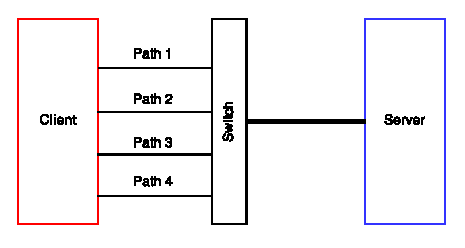
\includegraphics[width=0.8\textwidth]{images/perf-topo-phys.eps}
\caption{Physical topology inside mininet}
\label{fig:topo-phys}
\end{figure}

The corresponding logical topology is depicted on Figure \ref{fig:topo-log}. We are using 3 flows concurrently between the client and the server. The ITG application is sending traffic to one unique TUN interface and the traffic goes through our tunnel to reach the ITG receiver.

\begin{figure}[!ht]
\centering
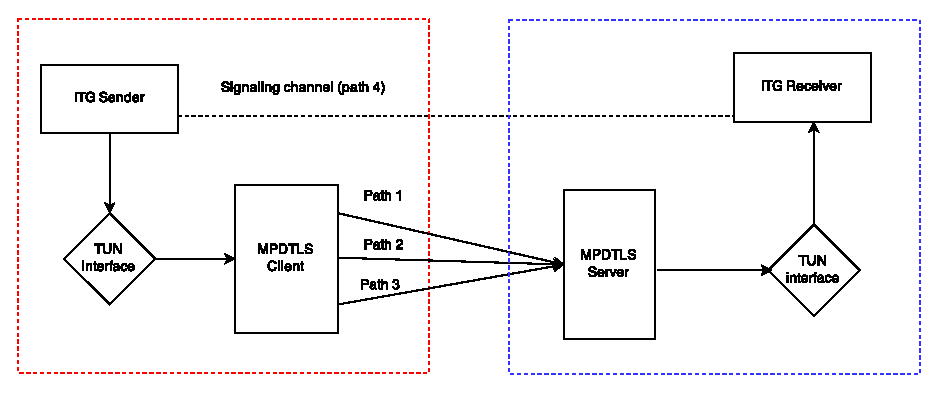
\includegraphics[width=\textwidth]{images/perf-topo-logic.eps}
\caption{Logical topology used for measurements}
\label{fig:topo-log}
\end{figure}

\subsection{Traffic balancing}

The first thing to evaluate is if we really take advantage of multiple interfaces and how we balance the traffic between them. We will run some experiments to determine in which conditions each scheduler performs well and how they compute the distribution of traffic in various environments.

\subsubsection{With dynamic bandwidth}

In this experiment, we have tested the two schedulers that are taking the context into consideration : \texttt{Optimize Latency} and \texttt{Optimize Loss}. The configuration used is the following (the path numbers are referring to Figure \ref{fig:topo-log}) :


\begin{table}[!ht]
\centering
\begin{tabular}{|c|c|c|c|}
\hline
Path n\degree & bandwidth & loss rate & delay  \\ \hline
1 &  1 Mbps & 0 & 10ms \\ \hline
2 & variable & 0 & 20ms \\ \hline
3 & not used & - & - \\ \hline
\end{tabular}
\end{table}

The goal is to modulate the bandwidth of B and see how its usage rate is impacted. We have generated constant traffic with D-ITG \cite{ditg} using both UDP and TCP. All these results are reported in Figure \ref{fig:dynbw}. The measures have been obtained during sessions of 60 seconds and every experiment has been repeated 11 times to evaluate the mean. The 95\% confidence interval of the mean is presented in white and has been computed with a Student T distribution.


\begin{figure}[!ht]
\centering
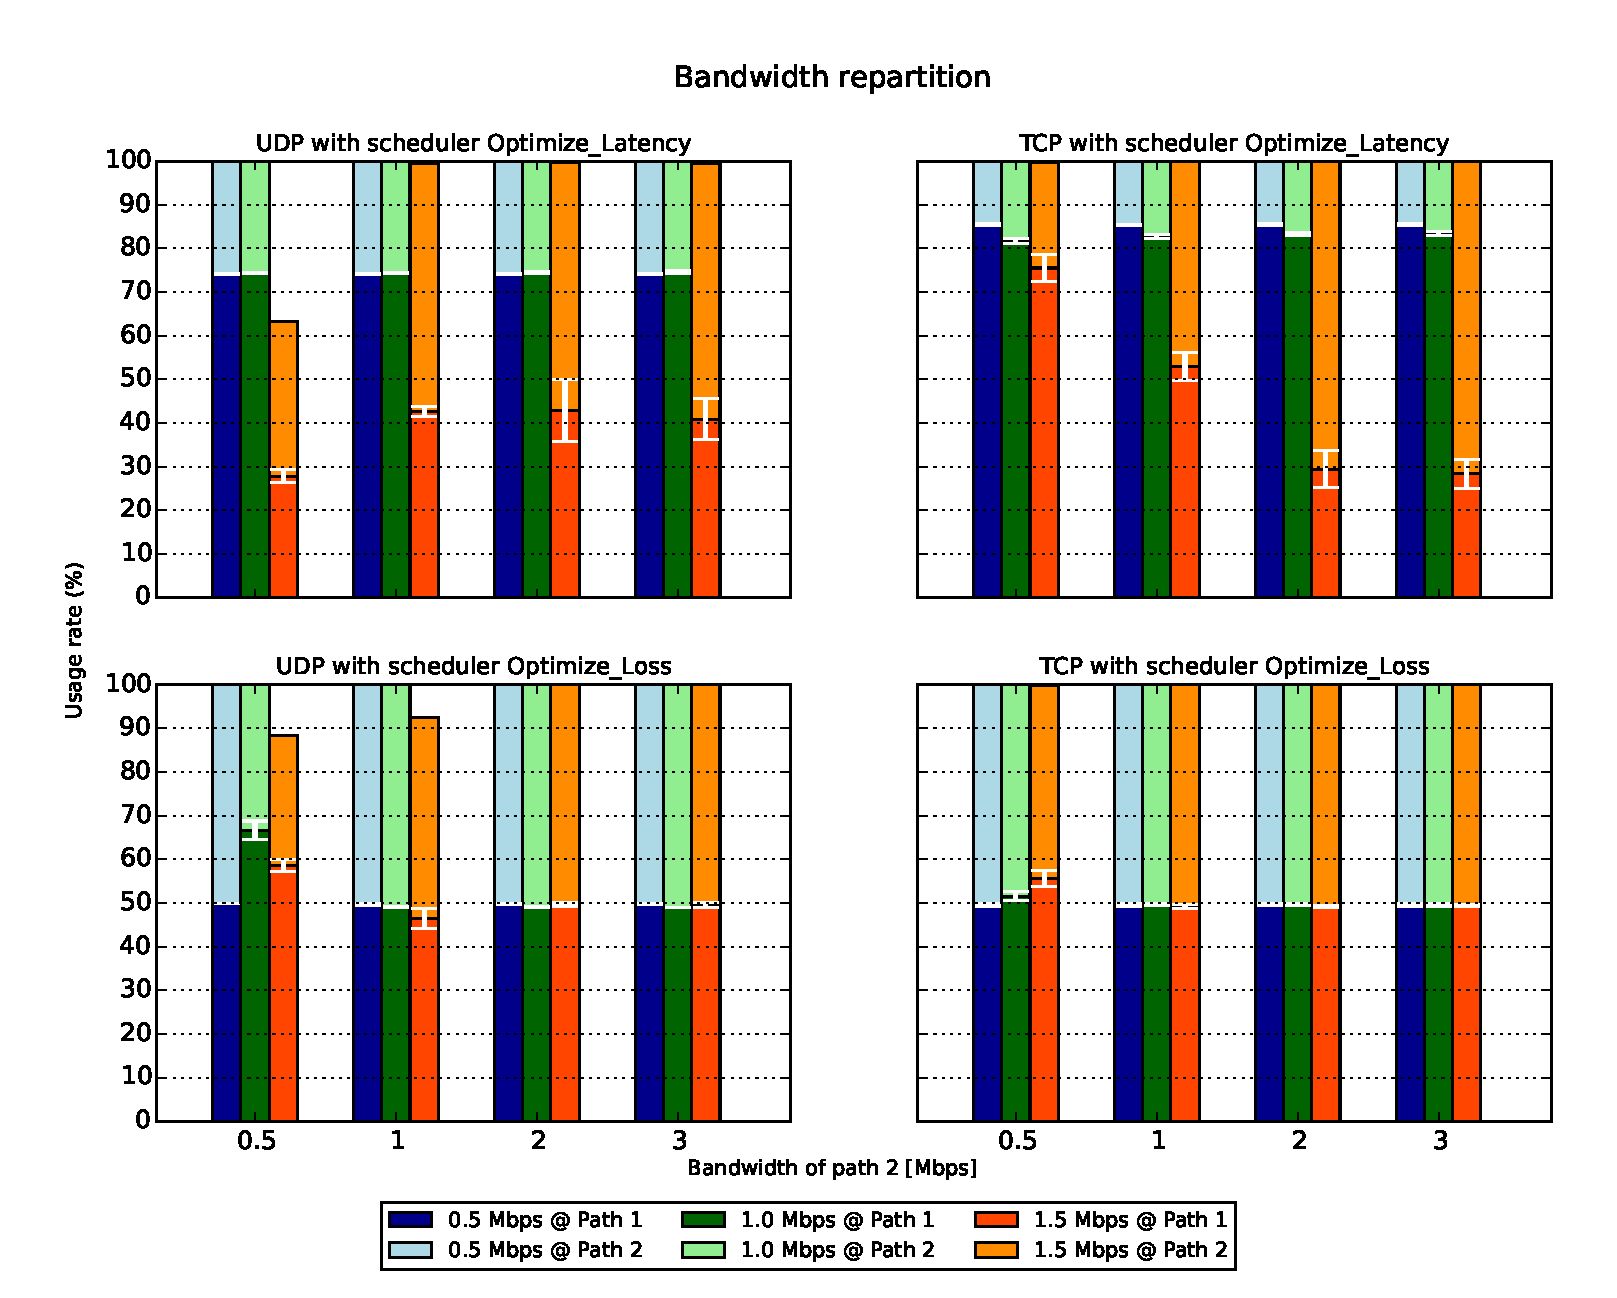
\includegraphics[width=\textwidth]{images/xp/graph1.eps}
\caption{Usage repartition with bandwidth variation}
\label{fig:dynbw}
\end{figure}


For every bandwidth value of path 2, we have 3 bars that represent the total amount of traffic we are trying to send through the tunnel. Each bar is separated in two parts that are showing the percentage of traffic passing through each path. The losses are easily identifiable because they occur every time the sum of the usage rates does not reach 100\%. Of course at the beginning we have congestion because if path 2 can support only $0.5Mbps$ then $bw(p1) + bw(p2) = 1.5Mbps$ and in the last case we are trying to send traffic at 1.5Mbps. So, it is supposed to use 100\% of the tunnel capacity which is impossible in practice due to our random scheduler. Moreover, this computation is not even taking into account the overhead introduced with the encapsulation inside DTLS. Indeed, we are sending packets of size 825 bytes inside the TUN interface and the resulting size of the DTLS \texttt{ApplicationData} packet is 905 bytes; so an overhead of almost 10\%.

First, it is interesting to confirm that the \texttt{Optimize loss} scheduler performs better if we are dealing with congested links and especially with UDP. Note that TCP doesn't experience losses the same way as UDP because it will reduce its emission rate internally with the congestion window mechanism. So even if we impose a certain amount of traffic, the real bandwidth will be lower with TCP in case of congestion.

Secondly, we observe a strange phenomenon if we look at the graph "UDP with scheduler Optimize Latency" : when we increase the total bandwidth to 1.5Mbps (orange), it does not optimize latency at all. Indeed, it gives only 28\% of the traffic to the faster link. We have tracked down the problem and it is apparently coming from a bad perception of the forward delay. At the beginning, it will use extensively path 1 as expected but will rapidly reach congestion as the capacity of path 1 is 1Mbps. The heartbeat messages that are used to evaluate the forward delay are themselves postponed by a few milliseconds due to this congestion and it is enough for the scheduler to estimate the delay is better on path 2. Even if later the forward delay is correctly estimated, we go back in the same cycle.  It is not the case with TCP at least at the beginning because TCP reduce the bandwidth to fit into the tunnel and therefore no congestion is observed.

\subsubsection{With dynamic loss rate}\label{sec:perfs-loss}

This time, we want to see how the schedulers will react if we progressively increase the loss rate of one of the path. The configuration is the following :

\begin{table}[!ht]
\centering
\begin{tabular}{|c|c|c|c|}
\hline
Path n\degree & bandwidth & loss rate & delay  \\ \hline
1 &  1 Mbps & 0 & 10ms \\ \hline
2 & 3 Mbps & variable & 10ms \\ \hline
3 & not used & - & - \\ \hline
\end{tabular}
\end{table}

Again we are using 2 paths only and they have the same latency but different bandwidth. We increase the loss rate of path 2 from 0\% to 3\% gradually. The results we have obtained are presented on Figure \ref{fig:dynloss}.


\begin{figure}[!ht]
\centering
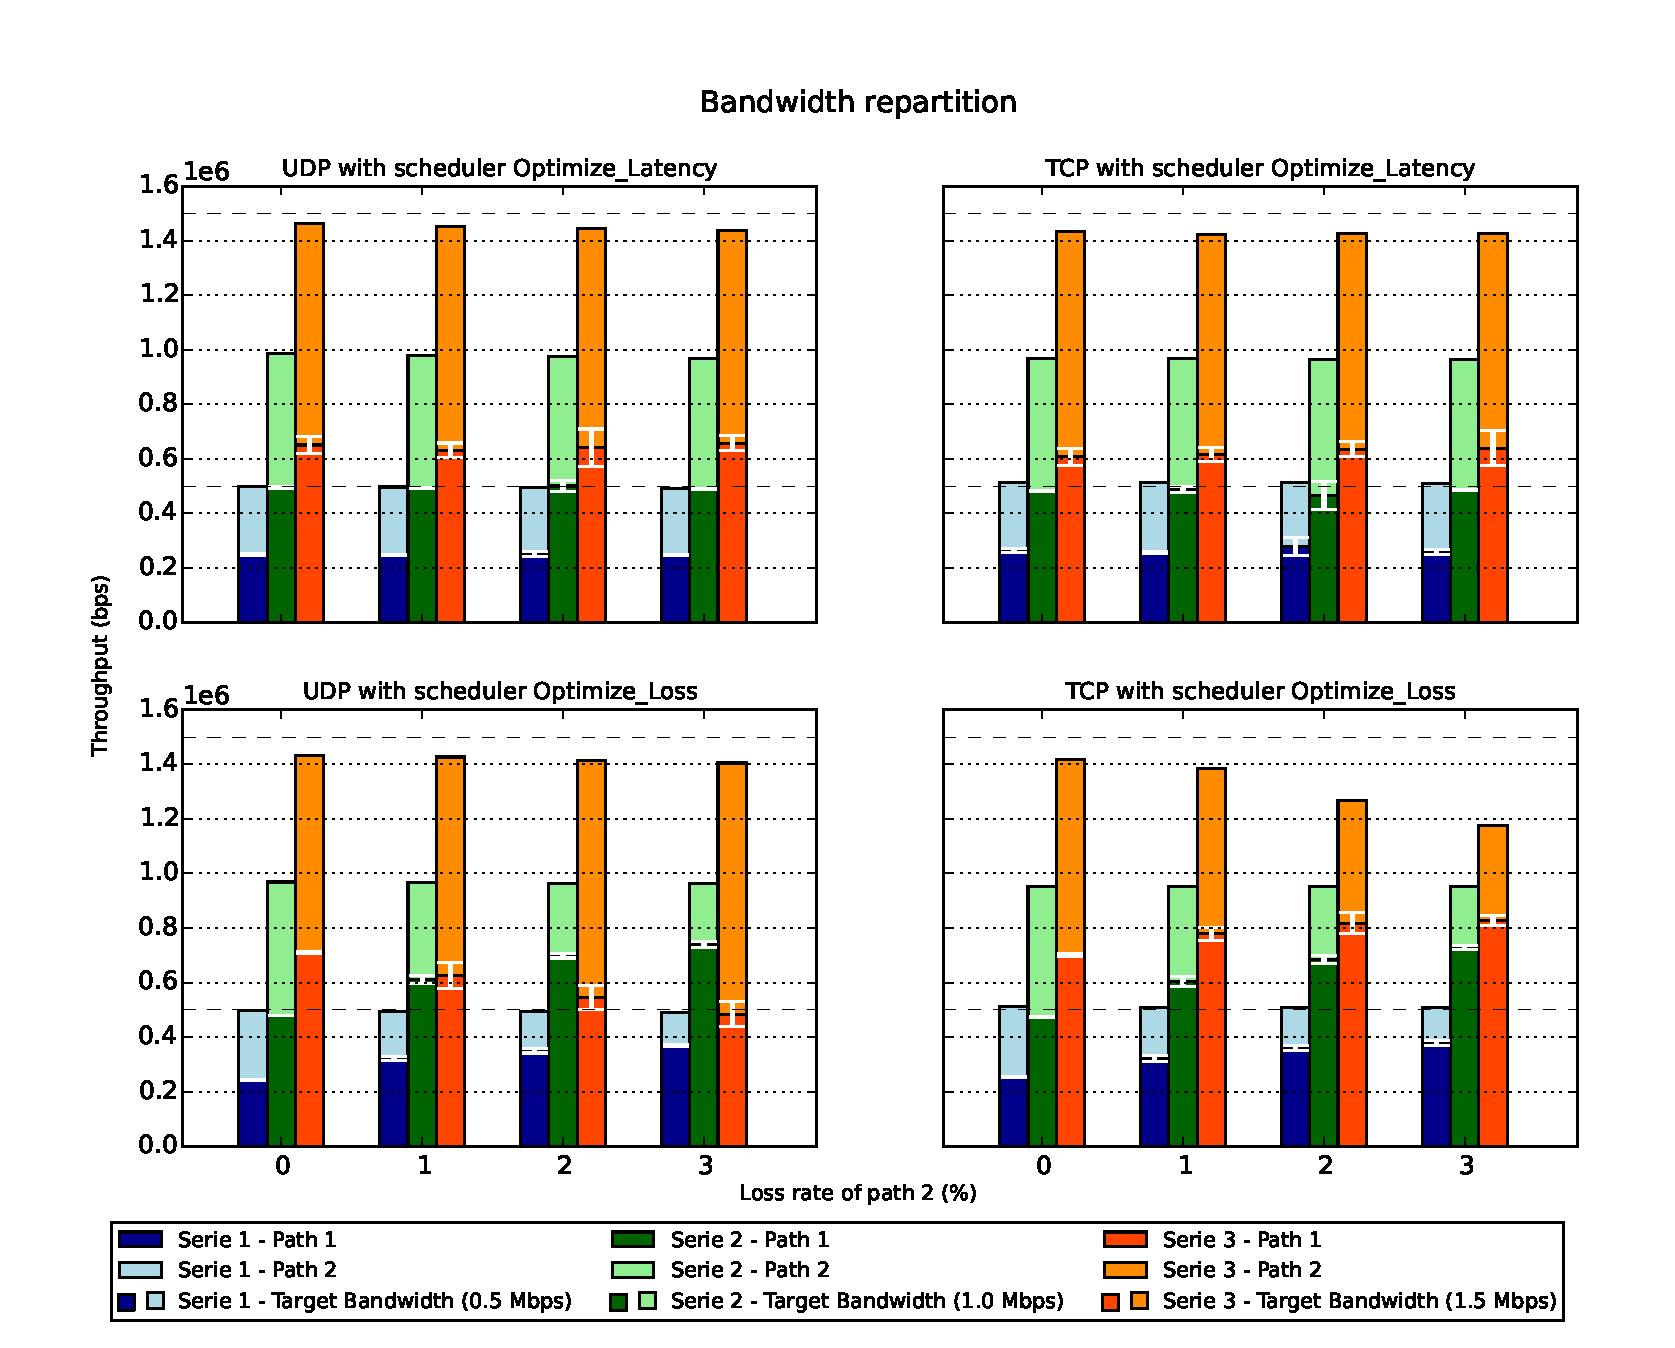
\includegraphics[width=\textwidth]{images/xp/graph2.eps}
\caption{Usage repartition with loss rate variation}
\label{fig:dynloss}
\end{figure}

A first thing to point out is the fact the scheduler \texttt{Optimize Latency} is not really impacted by the loss rate as we can expect. The proportion is always around 50\% for both TCP and UDP as the two links have the same delay. The little exception to this rule is noticed for the third bar (traffic at 1.5Mbps) probably because we reach the congestion limit on path 1. Therefore, the heartbeat messages are either delayed or dropped and the forward delay is overestimated.

On the other hand, the scheduler \texttt{Optimize loss} will progressively give more weight to the first path as it is loss free. We notice that UDP and TCP give different results concerning the latest bar which corresponds to the 1.5 Mbps transfer speed. Again, this can be explained by the congestion on path 1. UDP will keep sending packets even if they are dropped, therefore the scheduler will see important losses on path 1. The loss rate caused by congestion will overcome the one of path 2 and the scheduler will thus choose the best option among the two. However, for TCP, the congestion control mechanism will reduce the sending rate to avoid path 1 of being congested. In such conditions, path 1 remains the best option and thus is given more weight by the scheduler.


\subsection{Resiliency to interface removal}

The objective of the multipath is not only to do traffic balancing on exiting paths but also to modify dynamically the distribution of traffic if one interface becomes unavailable. For this experiment, we are using the topology of Figure \ref{fig:topo-log} with the following configuration : 

\begin{table}[!ht]
\centering
\begin{tabular}{|c|c|c|c|}
\hline
Path n\degree & bandwidth & loss rate & delay  \\ \hline
1 & 5 Mbps & 0 & 10ms \\ \hline
2 & 5 Mbps & 0 & 20ms \\ \hline
3 & 5 Mbps & 0 & 40ms \\ \hline
\end{tabular}
\end{table}

We will generate constant UDP traffic at 3 Mbps and observe the behavior of the implementation if the interface of path 1 is suddenly lost at $t=19s$. The bandwidth repartition is shown on Figure \ref{fig:xp-lossint-bw} and the scheduler used is \texttt{optimize loss}.


\begin{figure}[!ht]
\centering
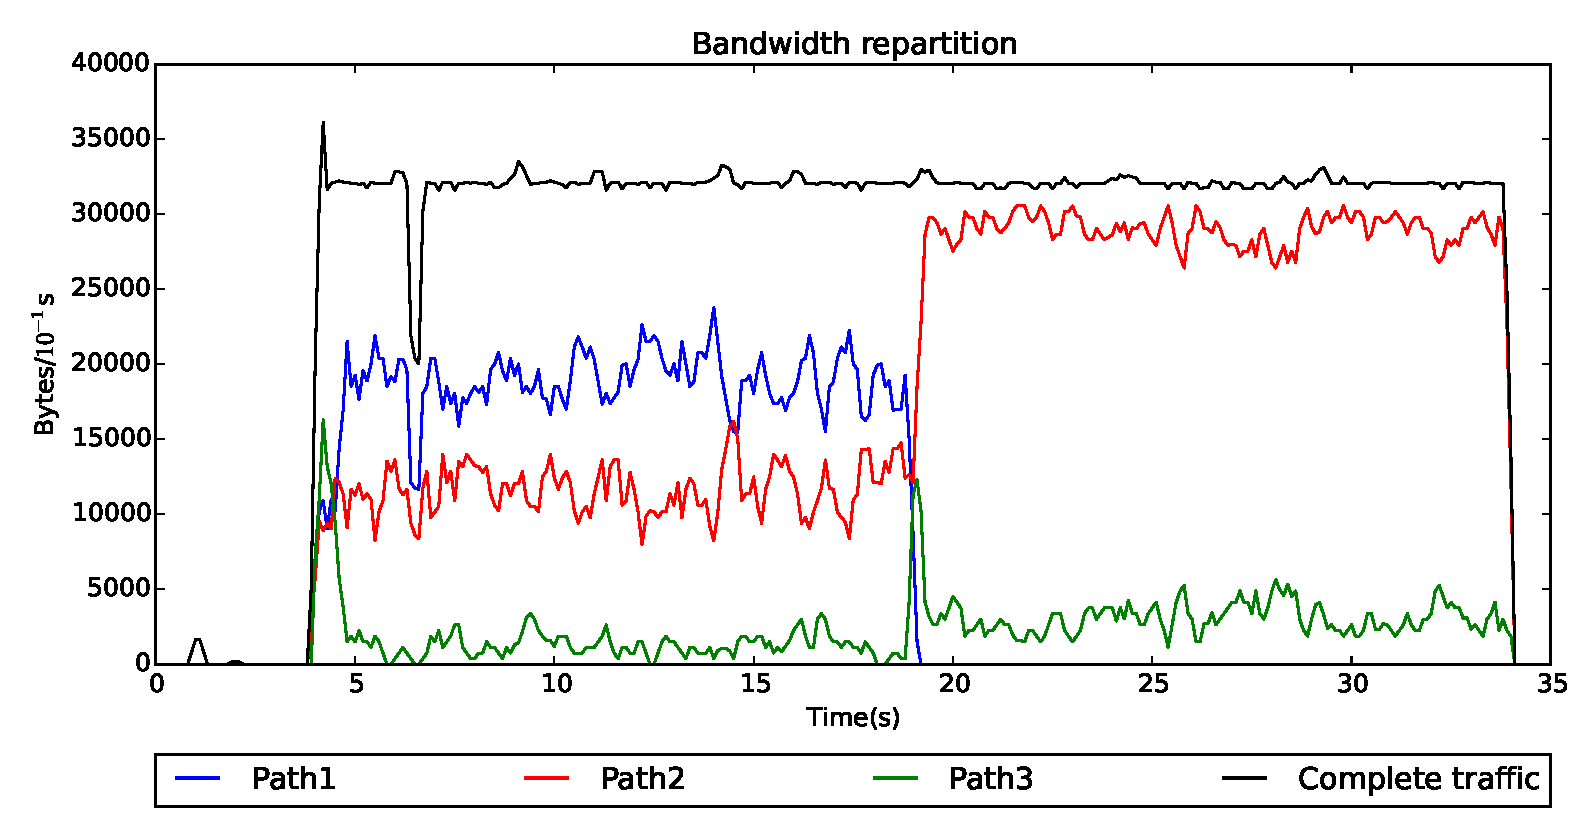
\includegraphics[width=\textwidth]{images/xp/intlost_bw.eps}
\caption{Reaction to interface removal}
\label{fig:xp-lossint-bw}
\end{figure}

Note that the path 1 was used for the handshake and we prove here that even if we remove our "primary" interface, the connection keeps going fluently. In the very first moments (at 4s), we see that the distribution is more or less equal between the flows. This setup time is needed to obtain some information about the forward delay. Heartbeat messages and feedback packets have to be exchanged between the two hosts. After 5 seconds, we see that the distribution is shaped with what we can expect from Equation \ref{eq:latency}: path 1 has almost $2/3$ of the traffic because he has the best delay, path 2 is still used because the difference of delays with path 1 is acceptable and then some traffic is given to path 3 to monitor the link.

When we loose the interface of path 1, the distribution is recomputed and most of the traffic will be re-routed to flow 2. Of course we are far from the congestion because each link has a bandwidth of 5 Mbps but the objective here was to see how the distribution is moving without other constraints. In this context, the scheduler is doing well by optimizing the overall latency as we can see in Figure \ref{fig:xp-lossint-delay}. After the loss of the fastest path, the overall delay is increased and is little above the  20ms threshold which is the delay of the new fastest link. We can also observe two peaks: the first one is due to the setup time and the second one is a temporary increase of path 3 usage to compensate the loss.



\begin{figure}[!ht]
\centering
\begin{minipage}{0.4\linewidth}
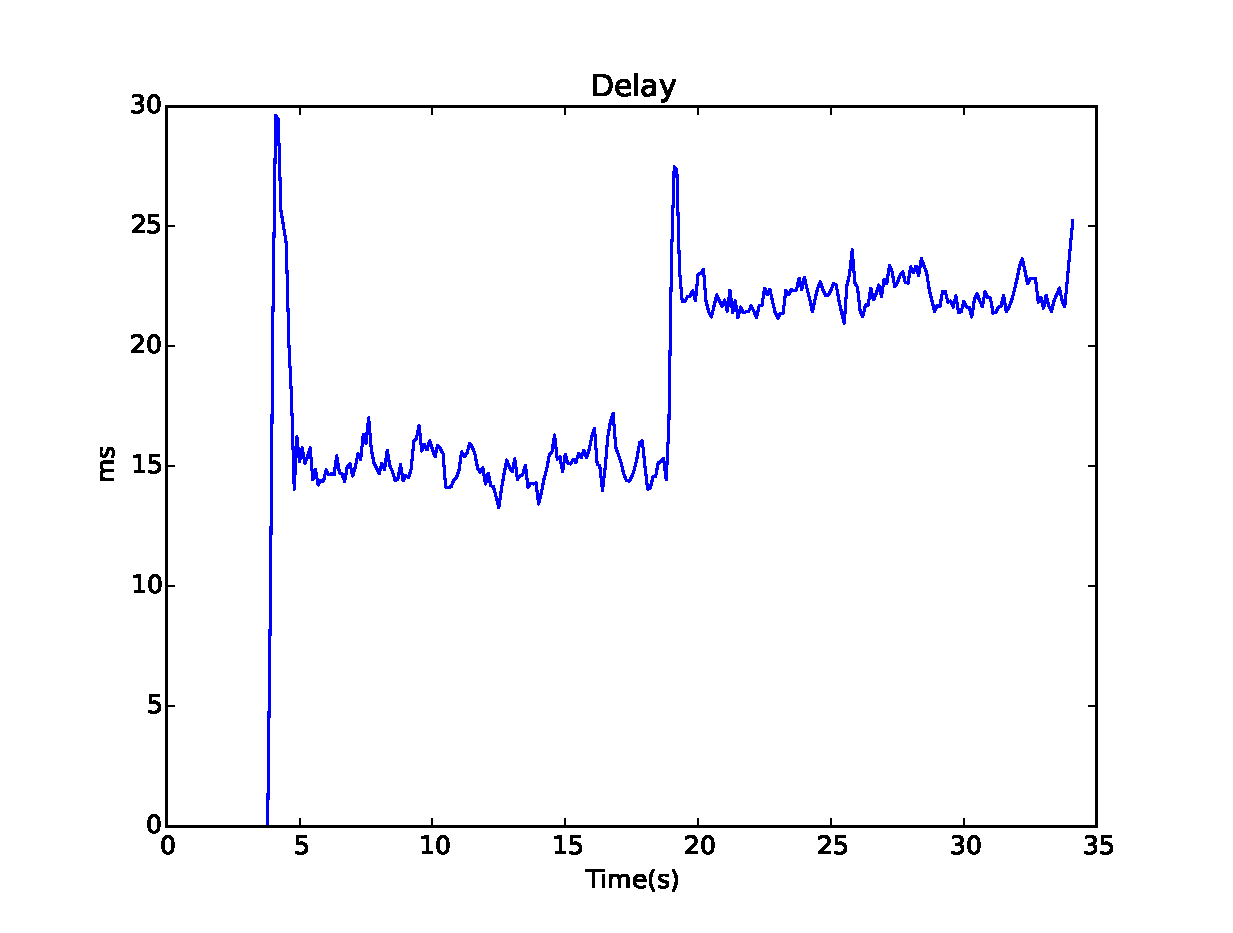
\includegraphics[width=\textwidth]{images/xp/intlost_delay.eps}
\caption{Overall delay}
\label{fig:xp-lossint-delay}
\end{minipage}
\begin{minipage}{0.59\linewidth}
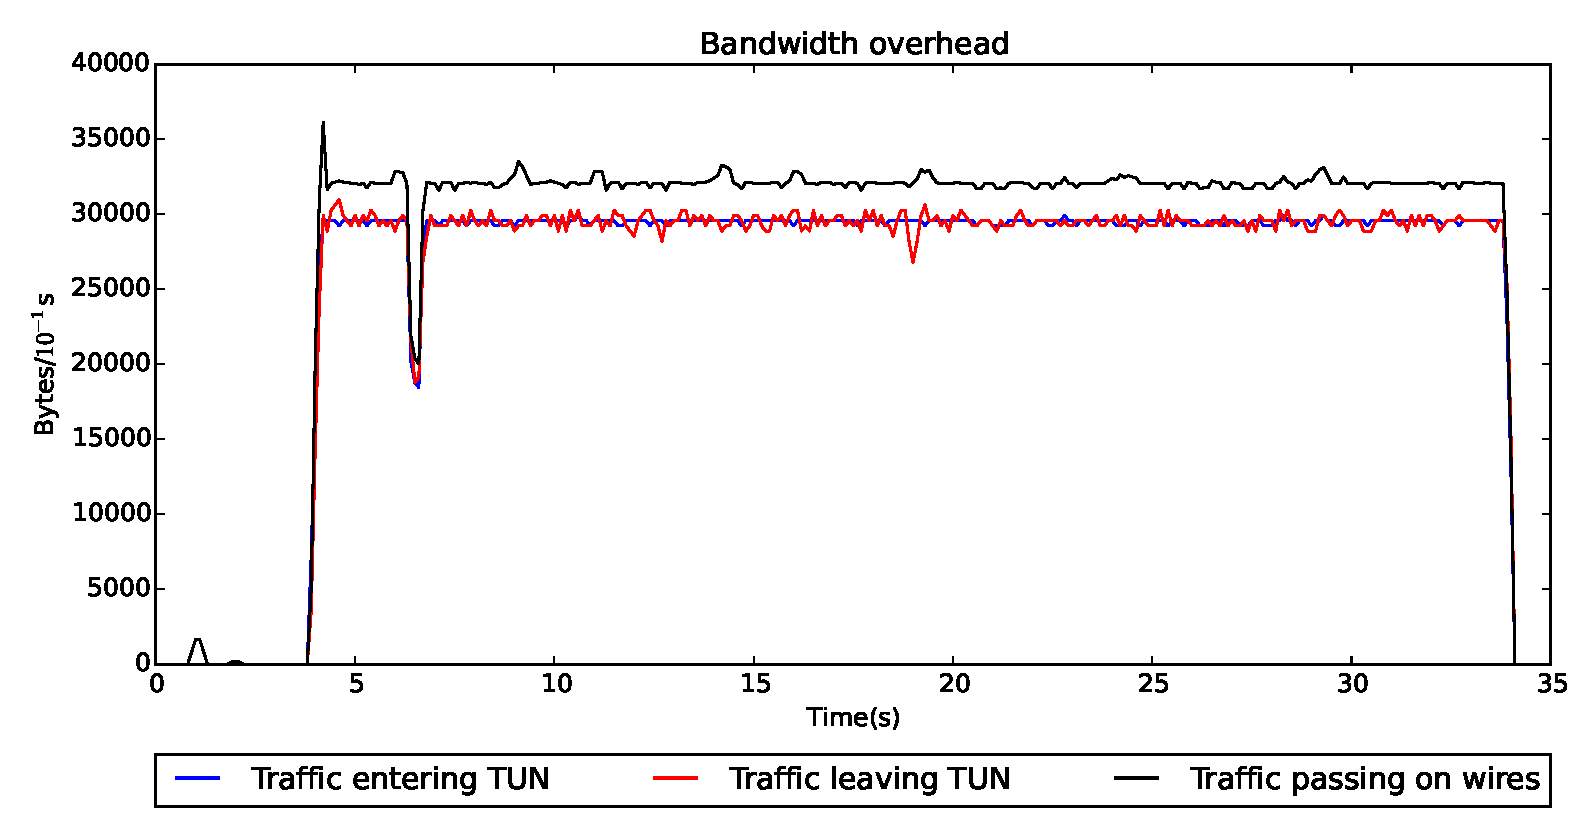
\includegraphics[width=\textwidth]{images/xp/intlost_tun.eps}
\caption{Application perception of traffic}
\label{fig:xp-lossint-tun}
\end{minipage}
\end{figure}

From the application point of view, the impact of such loss is shown in Figure \ref{fig:xp-lossint-tun}. We see in blue the traffic entering the tunnel which is constant here because we have parametrized D-ITG to do so, in red we see the traffic leaving the tunnel and in black we have the traffic generated by the tunnel. The difference between the blue and the black curve is the overhead caused by the encapsulation of D-ITG packets inside DTLS ones. Around the $19^{th}$ second, we notice a really small drop on the red curve, exactly when the interface was lost. This is the only thing the application will perceive from the loss of one interface. This is a huge improvement in comparison with a normal DTLS connection, which would ended the communication in case of such interface loss.

\begin{figure}[!ht]
\centering
\end{figure}

\subsection{Smooth add of a new interface}

In this section, we explore the reverse scenario: when one interface becomes available. At the beginning only path 1 and path 2 are available and at time $t=30s$ we add path 3. The configuration used is the following :

\begin{table}[!ht]
\centering
\begin{tabular}{|c|c|c|c|}
\hline
Path n\degree & bandwidth & loss rate & delay  \\ \hline
1 & 5 Mbps & 0 & 30ms \\ \hline
2 & 5 Mbps & 0 & 40ms \\ \hline
3 & 5 Mbps & 0 & 10ms \\ \hline
\end{tabular}
\end{table}

As we can see path 3 is faster and we expect it will take the lead over the two other ones. This is verified with our experiment as we can see on Figure \ref{fig:xp-addint-bw}. A significant portion of traffic is redirected through the new flow. At the beginning path 1 was the faster link so it was given the biggest part. But after the addition of the new interface, a re-computation is made according to equation \ref{eq:latency} and path 1 is less used.


\begin{figure}[!ht]
\centering
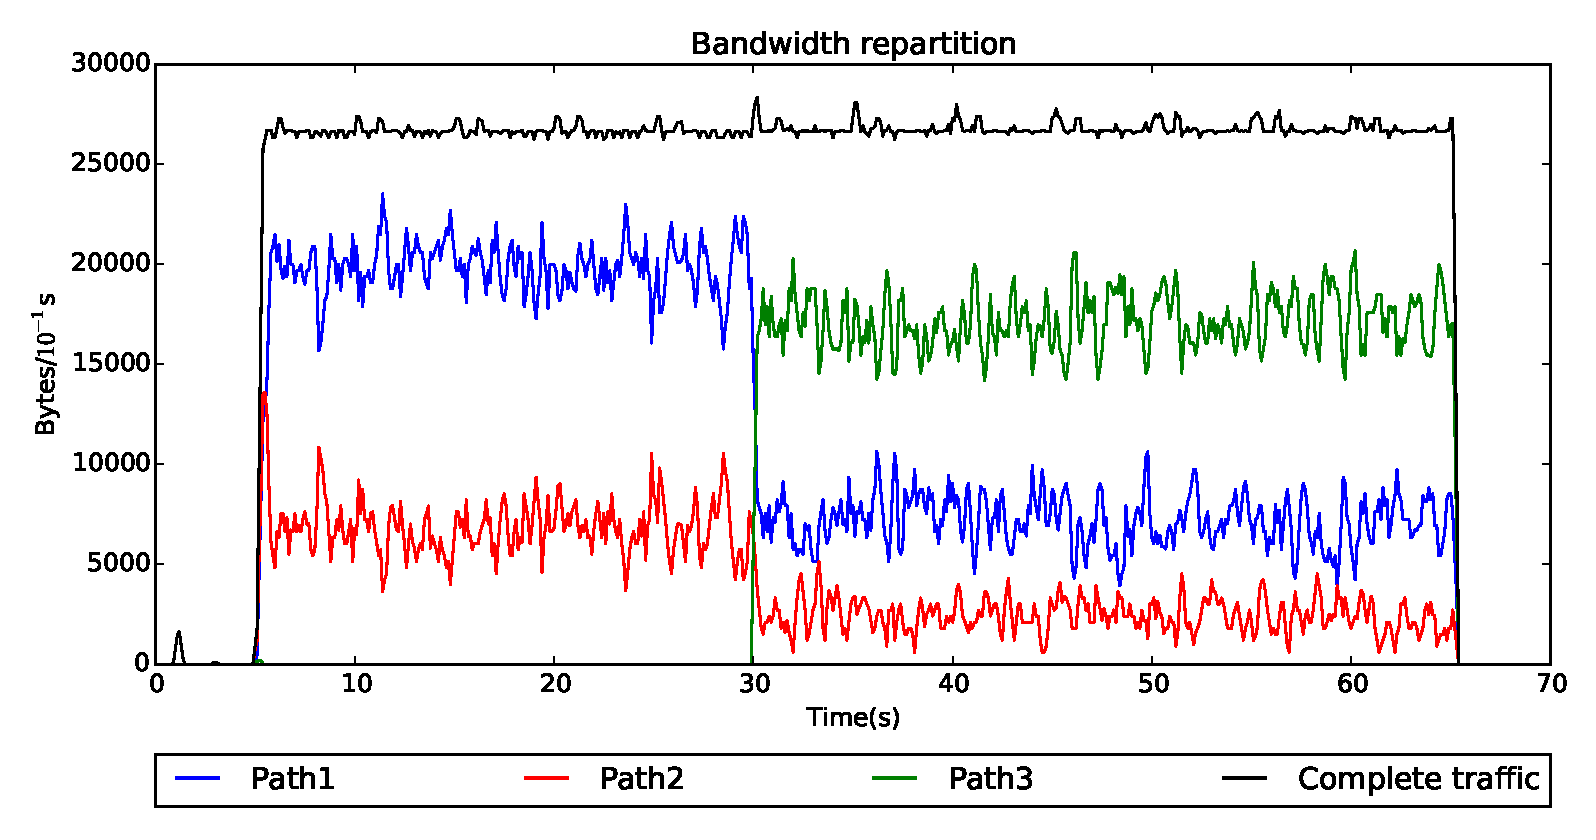
\includegraphics[width=\textwidth]{images/xp/addint_bw.eps}
\caption{Reaction to new interface addition}
\label{fig:xp-addint-bw}
\end{figure}

The overall delay is kept reasonably small according to Figure \ref{fig:xp-addint-delay} but we could probably optimize even more. That would imply putting more weight to path 1 and thus offload the two other flows. However this is a choice we have made to keep using all the paths while still trying to give more traffic to the faster link. It will allow for quicker recovery if the best interface is lost.

\begin{figure}[!ht]
\centering
\begin{minipage}{0.4\linewidth}
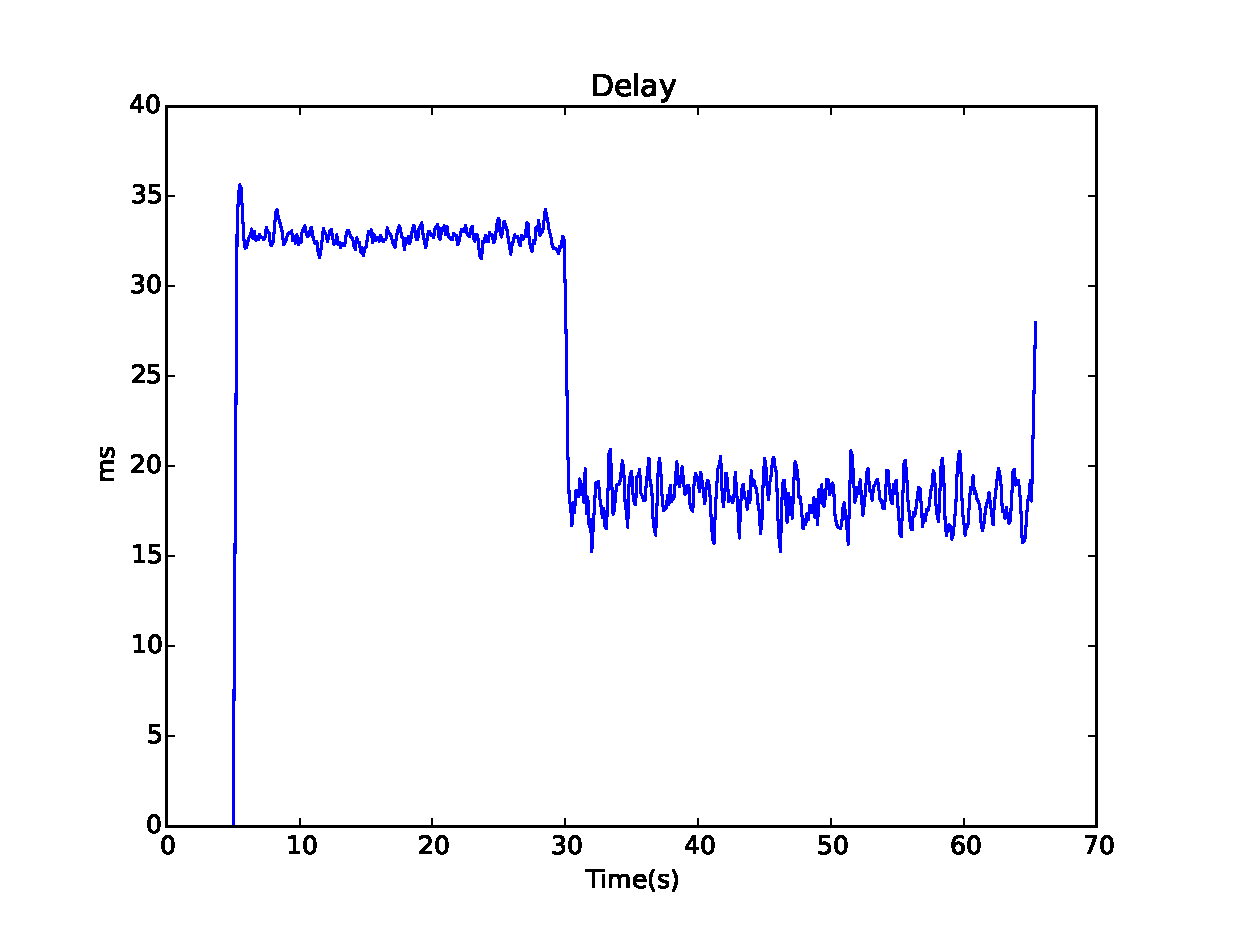
\includegraphics[width=\textwidth]{images/xp/addint_delay.eps}
\caption{Overall delay}
\label{fig:xp-addint-delay}
\end{minipage}
\begin{minipage}{0.59\linewidth}
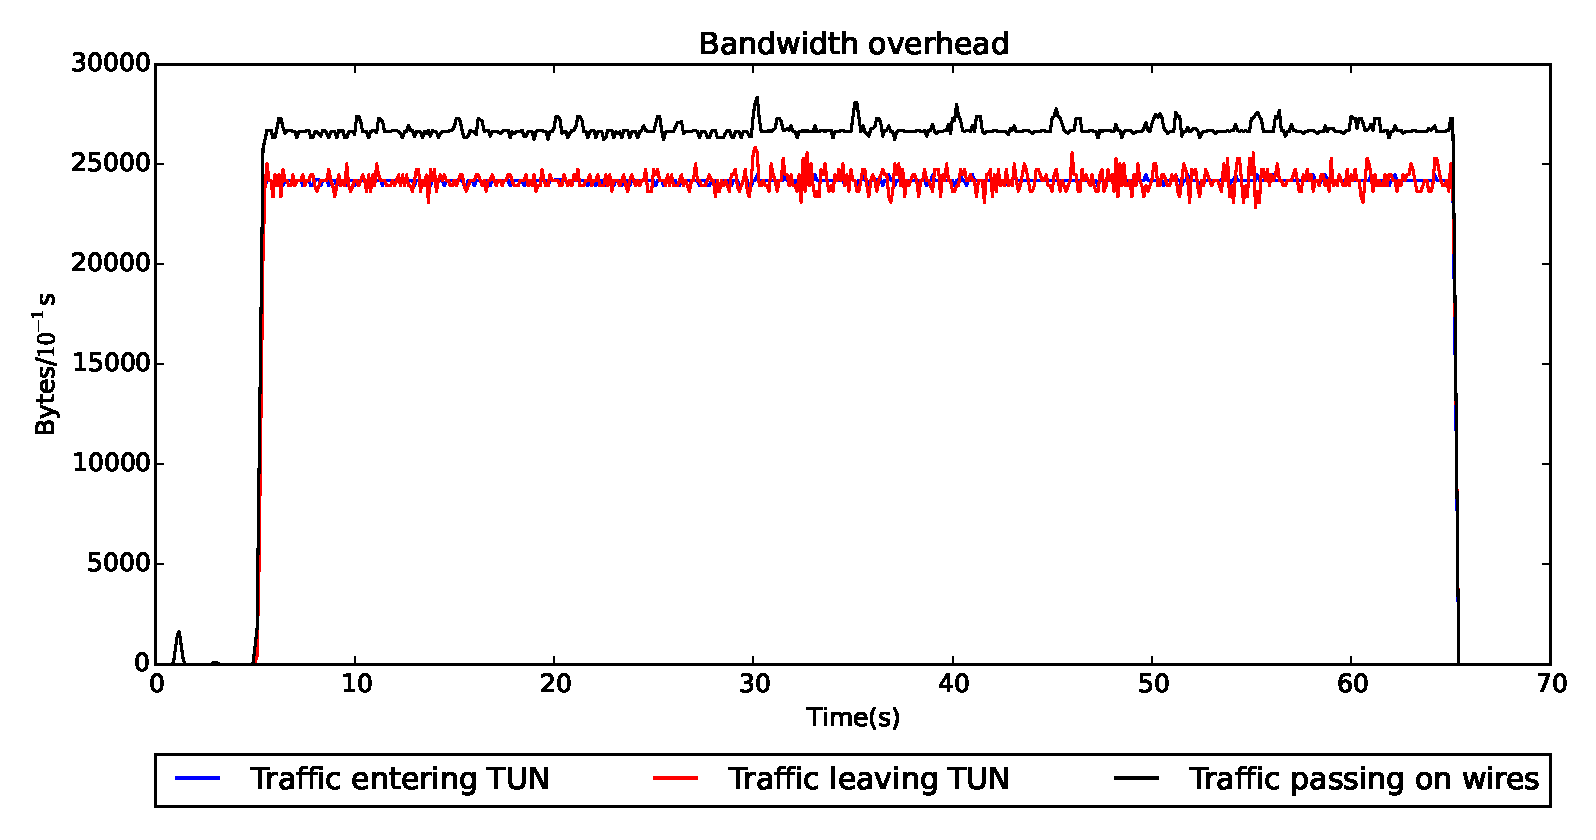
\includegraphics[width=\textwidth]{images/xp/addint_tun.eps}
\caption{Application perception of traffic}
\label{fig:xp-addint-tun}
\end{minipage}
\end{figure}

If we look at the traffic perceived by the application on Figure \ref{fig:xp-addint-tun}, we notice no real perturbation around $30s$. Although the traffic is a bit noisy after this time, this is explained by the fact we have 3 different paths with 3 different delays and therefore packets cannot arrive at a constant rate.

\section{Conclusion}

In this chapter, we have presented the VPN application we have designed to evaluate our MPDTLS implementation. To dispatch efficiently the packets between the available flows, 3 schedulers have been created : Round Robin, Optimize Loss and Optimize Latency. We have concentrated our evaluation on the last two since the round robin doesn't consider any contextual information. 

After various experiments, we have shown that the scheduler \texttt{Optimize Latency} behaves better when there is no congestion. Otherwise, it will try to push a great amount of traffic on the faster link and quickly triggers congestion. However, we have discovered that the counter-reaction will avoid too many losses : the additional delay caused by the congestion will increase the perceived latency. The scheduler will therefore redirect the traffic through other paths.

On the other hand, the scheduler \texttt{Optimize Loss} will behave better when there is congestion or simply if one link looses more packets than another one. This would typically be the case for a Wi-Fi interface in an environment with interferences. In such case, the more reliable link is preferred as long as it does not make the link congested.

In addition, we have shown that an application using our MPDTLS tunnel will not be troubled much if one interface is lost in the middle of the communication. This is also the case if we add a new interface on the fly.






 